%This is the first chapter of the dissertation

%The following command starts your chapter. If you want different titles used in your ToC and at the top of the page throughout the chapter, you can specify those values here. Since Columbia doesn't want extra information in the headers and footers, the "Top of Page Title" value won't actually appear.

\chapter[The ATLAS detector][Top of Page Title]{The ATLAS detector} \label{Chapter-ATLAS}

The dataset analyzed in this thesis was taken by the ATLAS detector \cite{PERF-2007-01}, which is located at the ``Point 1'' cavern of the LHC beampipe, just across the street from the main CERN campus.
The much-maligned acronym stands for \textit{A} \textit{T}oriodal \textit{L}HC \textit{A}pparatu\textit{S}.
ATLAS is a massive cylindrical detector, with a radius of 12.5 m and a length of 44 m, with nearly hermitic coverage around the collision point.
It consists of multiple subdetectors; each plays a role in ATLAS's ultimate purpose of measuring the energy, momentum, and type of the particles produced in collisions delivered by the LHC.
These subdetectors are immersed in a hybrid solenoid-toroid magnet system whichs forces charged particles to curve, which allows for precise measurements of their momenta.
These magnetic fields are maximized in the central solenoid magnet, which contains a magnetic field of $2$ T.
A schematic of the detector can be seen in \ref{fig:atlas_full}.

The \textit{inner detector} (ID) lies closest to the collision point, and contains three separate subdetectors.
It provides pseudorapidity\footnotemark coverage of $|\eta| < 2.5$ for charged particles to interact with the tracking material.
\footnotetext{ATLAS uses a right-handed Cartesian coordinate system; the origin is defined by the nominal beam interaction point.
The positive-$z$ direction is defined by the incoming beam travelling counterclockwise around the LHC.
The positive-$x$ direction points towards the center of the LHC ring from the origin, and the positive-$y$ direction points upwards towards the sky.
For particles of transverse (in the $x-y$ plane) momentum $p_T = \sqrt{p_x^2 + p_y^2}$ and energy $E$, it is generally most convenient fully describe this particle's kinematics as measured by the detector in the $(p_T, \phi, \eta, E)$ basis.
The angle $\phi = \arctan(p_y/p_x)$ is the standard azimuthal angle, and $\eta = \ln{\tan(\theta/2)} $ is known as the pseudorapidity, and defined based on the standard polar angle $\theta = \arccos(p_z/p_T)$.
For locations of i.e. detector elements, both $(r, \phi, \eta)$ and $(z, \phi, \eta)$ can be useful.}
The tracks reconstructed from the inner detector hits are used to reconstruct the primary vertices, as noted in Ch.\ref{ch:lhc}, and to determine the momemta of charged particles.
The ATLAS \textit{calorimeter} consists of two subdetectors, known as the \textit{electromagnetic} and \textit{hadronic} calorimeters.
These detectors stop particles in their detector material, and measure the energy deposition inside, which measures the energy of the particles deposited.
The calorimeters provide coverage out to pseudorapidity of $|\eta| < 4.9$.
The muon spectrometer is aptly named; it is specifically used for muons, which are the only particles which generally reach the outer portions of the detector.
In this region, we have the large tracking systems of the muon spectrometer, which provide precise measurements of muon momenta.
The muon spectrometer has pseudorapidity coverage of $|\eta| < 2.7$.

\begin{figure}
\caption{The ATLAS detector} \label{fig:atlas_full}
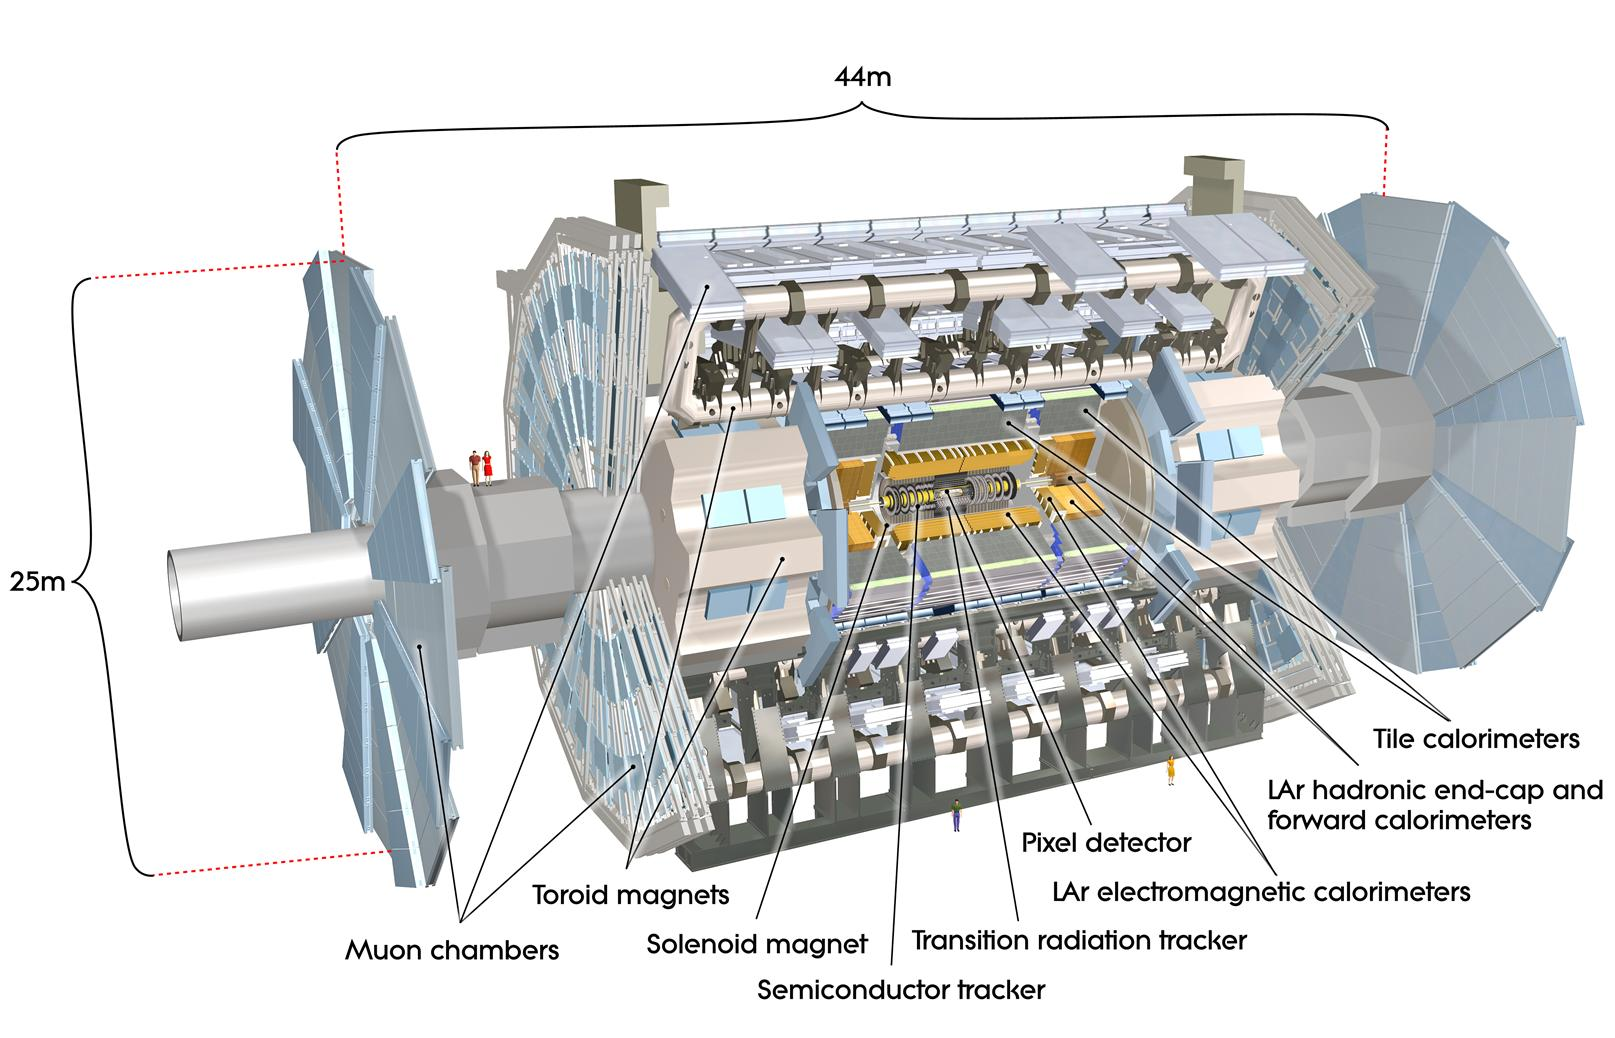
\includegraphics[width=.9\linewidth]{atlas_full}
\end{figure}

\section{Magnets}

\begin{figure}
\caption{The ATLAS magnet system} \label{fig:atlas_magnets}
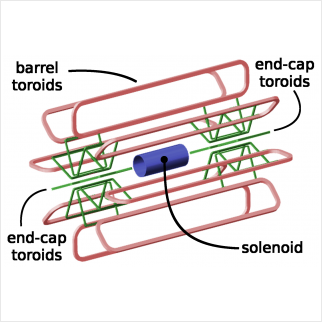
\includegraphics[width=.9\linewidth]{atlas_magnets}
\end{figure}

ATLAS contains multiple magnetic systems; primarily, we are concerned with the solenoid, used by the inner detector, and the toroids located outside of the ATLAS calorimeter.
A schematic is shown in Fig.\ref{fig:atlas_magnets}.
These magnetic fields are used to bend charged particles under the Lorentz force, which subsequently allows one to measure their momentum.

The ATLAS central solenoid \cite{Yamamoto:2008zze} is a 2.3 m diameter, 5.3 m long solenoid at the center of the ATLAS detector.
It produces a uniform magnetic field of 2 T; this strong field is necessary to accurately measure the charged particles in this field.
An important design constraint for the central solenoid was the decision to place it in between the inner detector and the calorimeters.
To avoid excessive impacts on measurements in the calorimetry, the central solenoid must be as transparent as possible\footnotemark.
\footnotetext{This is also one of the biggest functional differences between ATLAS and CMS; in CMS, the solenoid is outside of the calorimeters.}

The toroid system consists of eight air-core superconducting barrel loops; these give ATLAS its distinctive shape.
There are also two endcap air-core magnets.
These produce a magnetic field in a region of approximately 26 m in length and 10 m of radius.
The magnetic field in this region is non-uniform, due to the prohibitive costs of a solenoid magnet of that size.

\section{Inner Detector}

The ATLAS inner detector consists of three separate tracking detectors, which are known as, in order of increasing distance from the interaction point, the Pixel Detector \cite{Takubo:2014qsa}, Semiconductor Tracker (SCT) \todo{cite}, and the Transition Radiation Tracker (TRT) \todo{cite}.
\begin{figure}
\caption{The ATLAS inner detector} \label{fig:atlas_inner_detector}
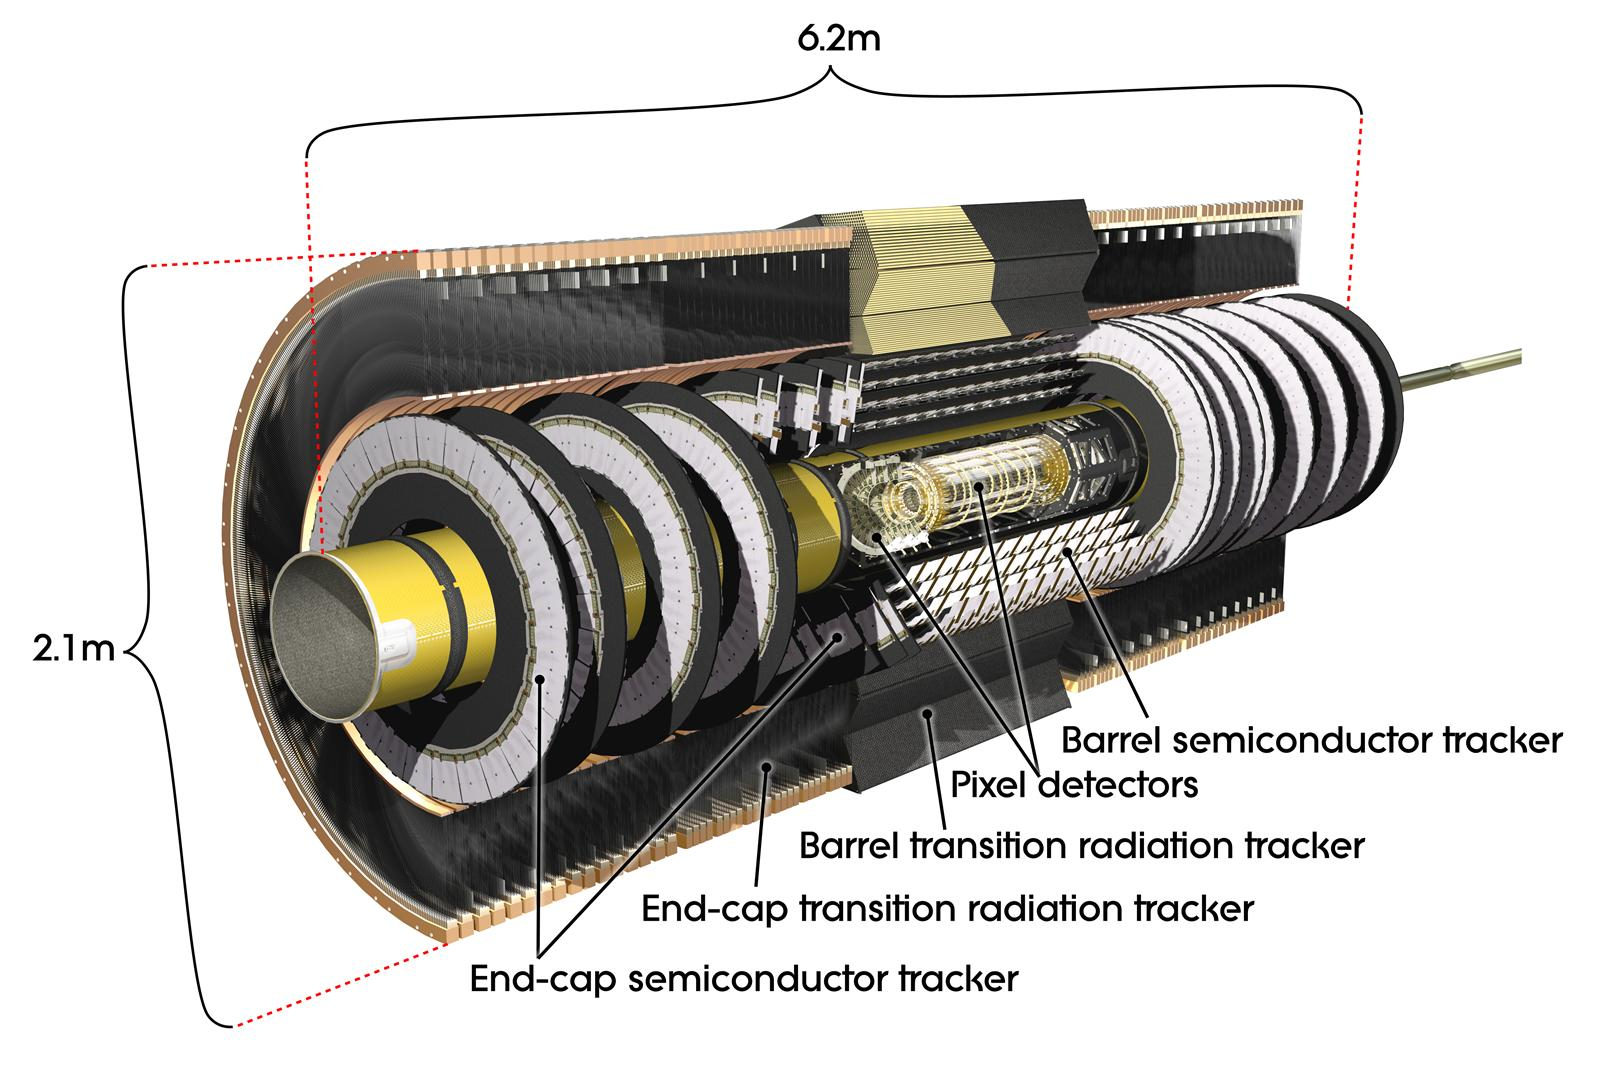
\includegraphics[width=.9\linewidth]{atlas_inner_detector}
\end{figure}
When charged particles pass through these tracking layers, they produce \textit{hits}, which using the known 2 T magnetic field, allows the reconstruction of \textit{tracks}.
Tracks are used as inputs for reconstruction of many higher-level physics objects, such as electrons, muons, photons, and \met.
Accurate track reconstruction is thus crucial for precise measurements of charged particles.

\subsection{Pixel Detector}
\todo{schematic}

The ATLAS pixel detector consists four layers of silicon ``pixels''.
This refers to the segmentation of the active medium into the pixels; compare to the succeeding silicon detectors, which will use silicon ``strips''.
This provides precise 3D hit locations.
The layers are known as the ``Insertable''\footnotemark B-Layer (IBL), the B-Layer (or Layer-0), Layer-1, and Layer-2, in order of increasing distance from the interaction point.
\footnotetext{\textit{Very} often, the IBL is mistakenly called the Inner B-Layer, which would have been a much more sensible name.}
These layers are very close to the interaction point, and therefore experience a large amount of radiation.

Layer-1, Layer-2, and Layer-3 were installed with the initial construction of ATLAS.
They contain front-end integrated electronics (FEI3s) bump-bonded to 1744 silicon modules; each module is 250 $\mu$m in thickness and contains 47232 pixels.
These pixels have planar sizes of 50 x 400 $\mu^2$ or  50 x 600 $\mu^2$, to provide highly accurate location information.
The FEI3s are mounted on long rectangular structures known as staves, which encircle the beam pipe.
A small tilt to each stave allows full coverage in $\phi$ even with readout systems which are installed.
These layers are at radia of 50.5 mm, 88.5 mm, and 122.5 mm from the interaction point.

The IBL was added to ATLAS after Run1 in 2012 at a radius of 33 mm from the interaction point.
The entire pixel detector was removed from the center of ATLAS to allow an additional pixel layer to be installed.
The IBL was required to preserve the integrity of the pixel detector as radiation damage leads to inoperative pixels in the other layers.
The IBL consists of 448 FEI4 chips, arranged onto 14 staves.
Each FEI4 has 26880 pixels, of planar size 50 x 250 $\mu$m.
This smaller granularity was required due to the smaller distance to the interaction point.

In total, a charged particle passing through the inner detector would expect to leave four hits in the pixel detector.

\subsection{Semiconductor Tracker}

\todo{schematic}
The SCT is directly beyond Layer-2 of the pixel detector.
This is a silicon strip detector, which do not provide the full 3D information of the pixel detector.
The dual-sensors of the SCT contain 2 x 768 individual strips; each strip has area 6.4 cm$^2$.
The SCT dual-sensor is then double-layered, at a relative angle of 40 mrad; together these layers provide the necessary 3D information for track reconstruction.
There are four of these double-layers, at radia of 284 mm, 355 mm, 427 mm, and 498 mm.
These double-layers provide hits comparable to those of the pixel detector, and we have four additional hits to reconstruct tracks for each charged particle.

\subsection{Transition Radiation Tracker}

The Transition Radiation Tracker is the next detector radially outward from the SCT.
It contains straw drift tubes; these contain a tungsten gold-plated wire of 32 $\mu$m diameter held under high voltage (-1530 V) with the edge of the Kapton-aluminum tube.
They are filled with a gas mixture of primarily xenon that is ionized when a charged particle passes through the tube.
The ions are collected by the ``drift'' due to the voltage inside the tubes, which is read out by the electronics.
This gives so-called ``continuous tracking'' throughout the tube, due to the large number of ions produced.

The TRT is so-named due to the \textit{transition radiation} (TR) it induces.
Due to the dielectric difference between the gas and tubes, TR is induced.
This is important for distinguishing electrons from their predominant background of minimum ionizing particles.
Generally, electrons have a much larger Lorentz factor than minimum ionizing particles, which leads to additional TR.
This can be used as an additional handle for electron reconstruction.
\missingfigure{TRT schematic}

\section{Calorimeter}

\begin{figure}
\caption{The ATLAS calorimeter} \label{fig:atlas_calorimeter}
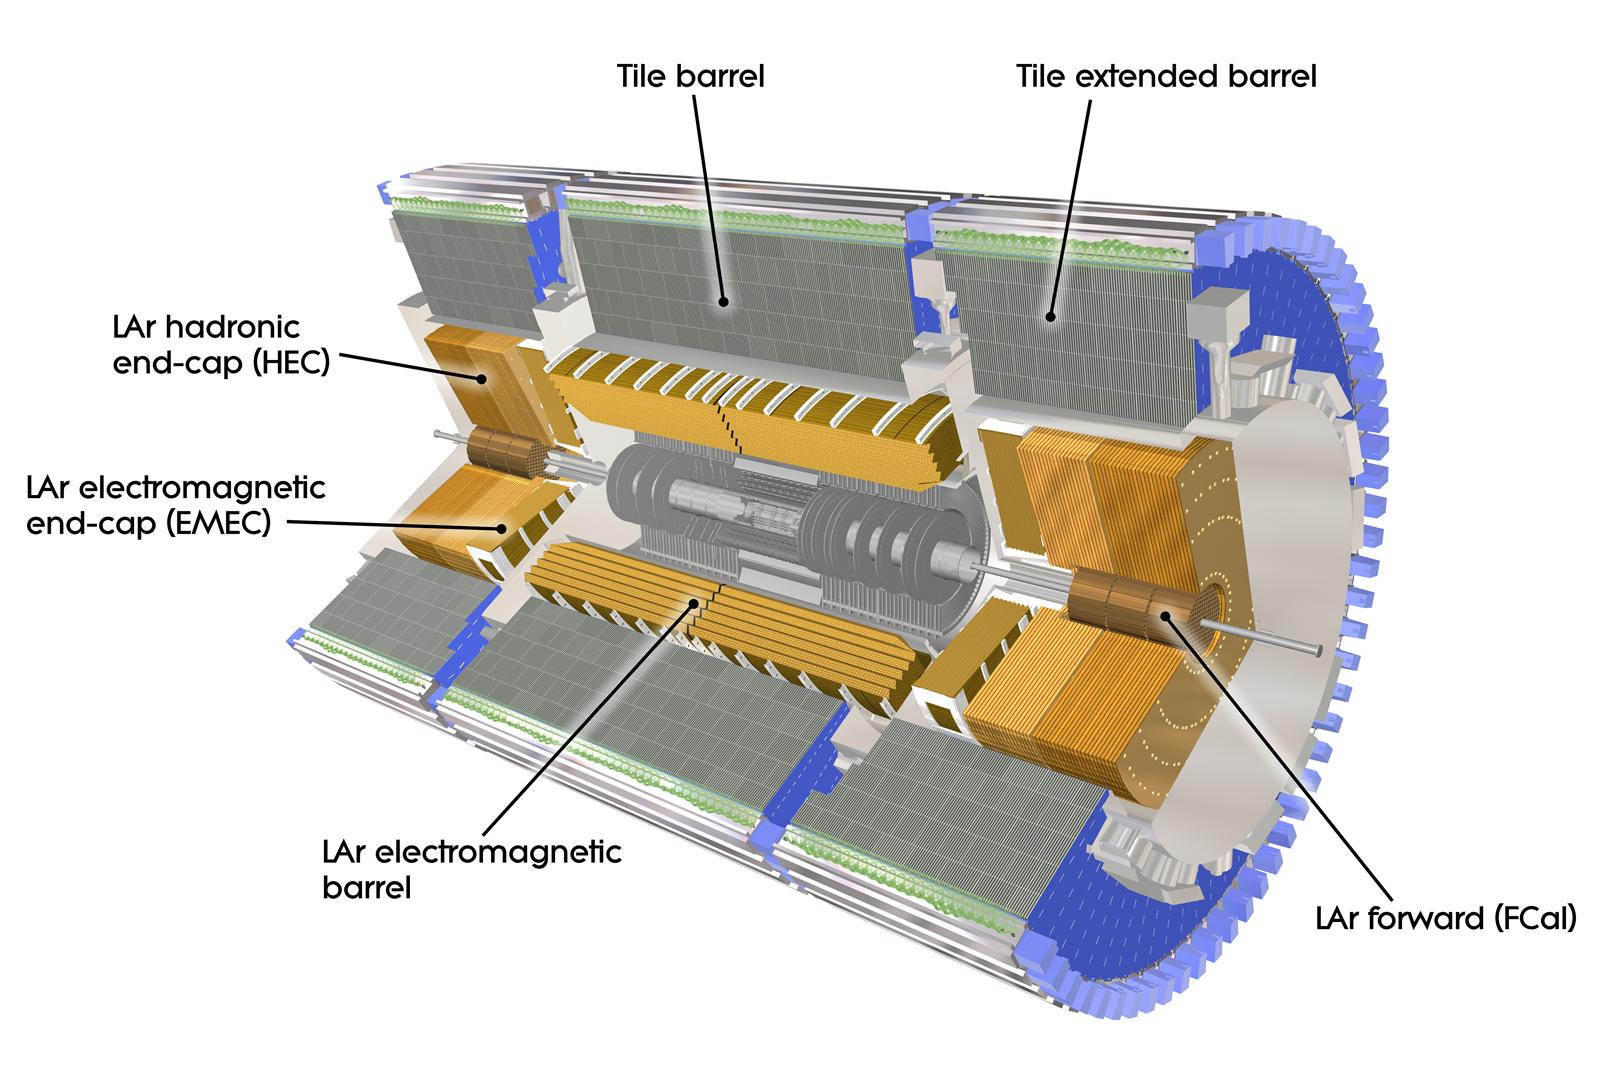
\includegraphics[width=.9\linewidth]{atlas_calorimeter}
\end{figure}


\subsection{Electromagnetic Calorimeter}

\subsection{Hadronic Calorimeter}

\section{Muon Spectrometer}


\begin{figure}
\caption{The ATLAS muon spectrometer} \label{fig:atlas_muon_spectrometer}
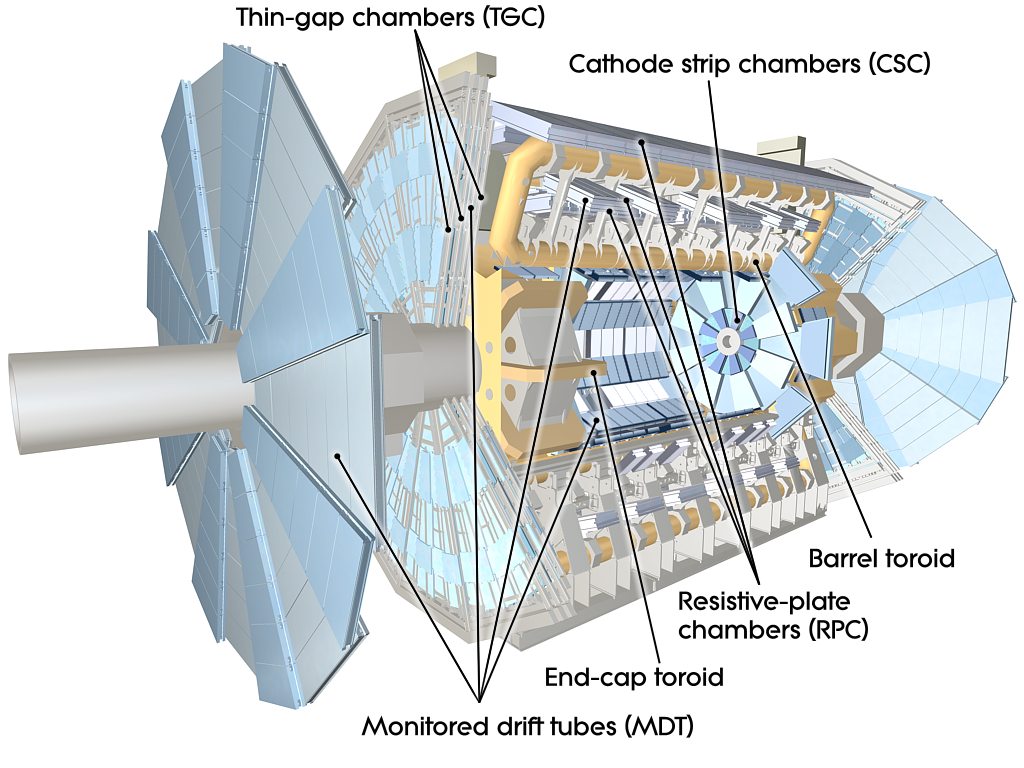
\includegraphics[width=.9\linewidth]{atlas_muon_spectrometer}
\end{figure}


\section{Trigger System}